\documentclass[cn,11pt]{elegantbook}

\title{光学工程基础复习}
\subtitle{专业课程知识点总结}

\author{Keiyui Kwan}
\institute{Zhejiang University}
\date{\today}
\version{1.00}

\extrainfo{God said, "Let there be light", and there was light.}

\logo{logo.png}
\cover{cover.jpg}

\begin{document}
	
\maketitle
\tableofcontents
	
% \thispagestyle{empty}
	
\mainmatter
\hypersetup{pageanchor=true}
	
\chapter*{序言}
\addcontentsline{toc}{chapter}{序言}
\markboth{序言}{}
欢迎阅读本书,本书进行书写时参考的资料主要为天津大学郁道银等编著的《工程光学(第四版)》以及浙江大学李晓彤等编著的《几何光学·像差·光学设计(第三版)》。本书使用\LaTeX 进行写作,模板采用的是Elegant\LaTeX 系列模板中的\href{https://github.com/ElegantLaTeX/ElegantBook}{ElegantBook}。以下为我的联系方式:
\begin{itemize}
	\item 个人网站:\href{https://guanqr.com/}{https://guanqr.com/}
	\item GitHub 网址:\href{https://github.com/guanqr/}{https://github.com/guanqr/}
	\item E-mail:\email{guanqirui@zju.edu.cn}
\end{itemize}

\chapter{理想光学系统}

\begin{introduction}
	\item 物像共轭关系(定义\ref{def:conjugate})
	\item 基点和基面(第\ref{subsect:base-point}节)
	\item 光学系统的节点(第\ref{subsect:node}节)
	\item 光学系统的组合(第\ref{sect:combination-of-optical-systems}节)
	\item 光焦度(定义\ref{def:focal-power})
	\item 视觉放大率(定义\ref{def:visual-magnification})
\end{introduction}

将光学系统在近轴区完善成像的理论推广到任意大的空间,以任意宽的光束都成完善像的光学系统称为理想光学系统。共轴理想光学系统又称为高斯光学。

\section{理想光学系统与共线成像理论}

\begin{definition}{物像共轭关系}{int}\label{def:conjugate}
	在理想光学系统中,任何一个物点发出的光线在系统的作用下所有的出射光线仍然相交于一点。由光路的可逆性和折射、反射定律中光线方向的确定性,可得出每一个物点对应于唯一一个像点。通常将这种物像对应关系叫做“共轭”。
\end{definition}

如果光学系统的物空间和像空间都是均匀透明介质,则入射光线和出射光线均为直线,根据光线的直线传播定律,由符合点对应点的物像空间关系可以推论出直线成像为直线、平面成像为平面的性质。这种点对应点、直线对应直线、平面对应平面的成像变换称为共线成像。

\begin{property}
共轴理想光学系统所成的像的性质:
\begin{enumerate}
	\item 位于光轴上的物点对应的共轭像点必然位于光轴上;位于过光轴的某一个截面内的物点对应的共轭像点必然位于该平面的共轭像面内;同时,过光轴的任意截面成像性质是相同的。
	\item 垂直于光轴平面物所成的共轭平面像的几何形状完全与物相似,在整个物平面上无论哪一部分,物和像的大小比例均等于常数。
	\item 一个共轴理想光学系统,如果已知两对共轭面的位置和放大率,或者一对共轭面的位置和放大率,以及轴上的两对共轭点的位置,则其他一切物点的像点都可以根据这些已知的共轭面和共轭点来表示。
\end{enumerate}
\end{property}

\section{理想光学系统的基点与基面}
\subsection{无限远的轴上物点对应的像点$F'$}
\label{infty-object}

\begin{enumerate}	
	\item 无限远轴上物点发出的光线:
	
	设$h$为轴上物点$A$发出的一条入射光线的投射高度,由三角关系近似有
	\begin{equation}
		\tan U=\frac{h}{L}
	\end{equation}
	式中,$U$为孔径角,$L$为物方截距。当$L$趋于无穷大时,物点$A$向无限远处左移,$U$趋于$0$,即无穷远轴上物点发出的光线都与光轴平行。
	\item 像方焦点、焦平面;像方主点、主平面:
	
	如图\ref{perfect-optical-system}所示,平行于光轴的入射光线$AE_1$通过理想光学系统后,出射光线$G'F'$交光轴于$F'$。$F'$为无限远轴上物点的像点,称为像方焦点。过$F'$作垂直于光轴的平面,称为像方焦平面。像方焦平面与无限远处垂直于光轴的物平面共轭。
	
	\begin{figure}[htbp]
		\centering
		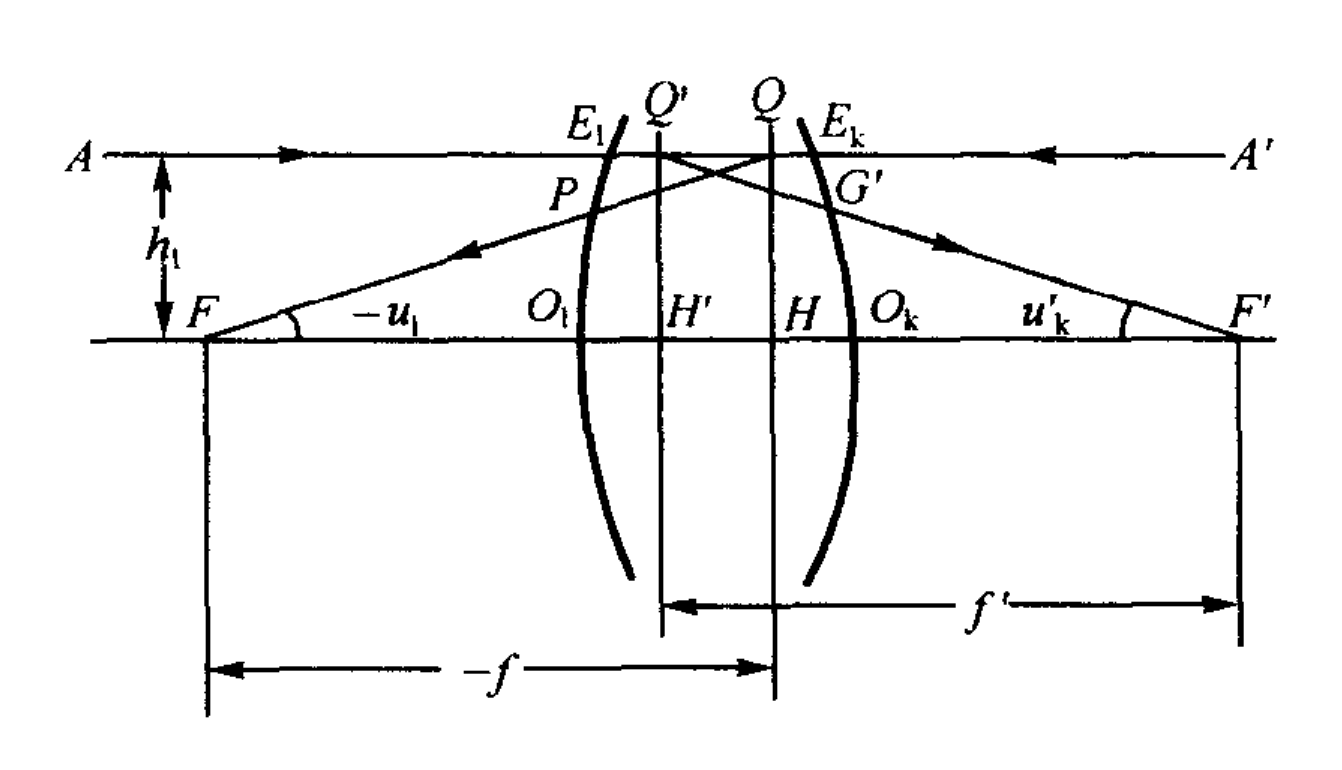
\includegraphics[width=0.6\textwidth]{perfect-optical-system.png}
		\caption{理想光学系统}
		\label{perfect-optical-system}
	\end{figure}
	
	入射光线$AE_1$的延长线与出射光线$G'F'$的反向延长线交于一点$Q'$,过$Q'$作垂直于光轴的平面交光轴于$H'$点,则$H'$点为像方主点,$Q'H'$平面为像方主平面,从主点$H'$搭配焦点$F'$之间的距离为像方焦距$f'$。有
	\begin{equation}
		f'=\frac{h}{\tan U'}
	\end{equation}
	
	\item 无限远轴外物点发出的光线:
	
	进入光学系统的光线总是相互平行的,且与光轴有一定夹角$\omega$。这一束光线经过系统后,一定交于像方焦平面的某一点,这一点为无限远轴外物点的共轭像点。	
\end{enumerate}

\subsection{无限远轴上像点对应的物点$F$}
相关概念同第\ref{infty-object}节内容。物方焦平面上任意一点发出的光线,通过理想光学系统后亦是一组相互平行的光线。
\subsection{物方主平面与像方主平面间的关系,理想光学系统的基点和基面}
\label{subsect:base-point}
如图\ref{perfect-optical-system}所示,两条入射光线$AE_1$和$FP$都经过$Q$,相应地出射光线都经过$Q'$,$Q$和$Q'$为共轭点,因此物方主平面和像方主平面是一对共轭面,垂轴放大率为$+1$。

\begin{definition}{基点和基面}{int}
	一对主点和主平面,一对焦点和焦平面,称为共轴理想光学系统的基点和基面。
\end{definition}

\section{理想光学系统的物像关系}
\subsection{牛顿公式}
\begin{figure}[htbp]
	\centering
	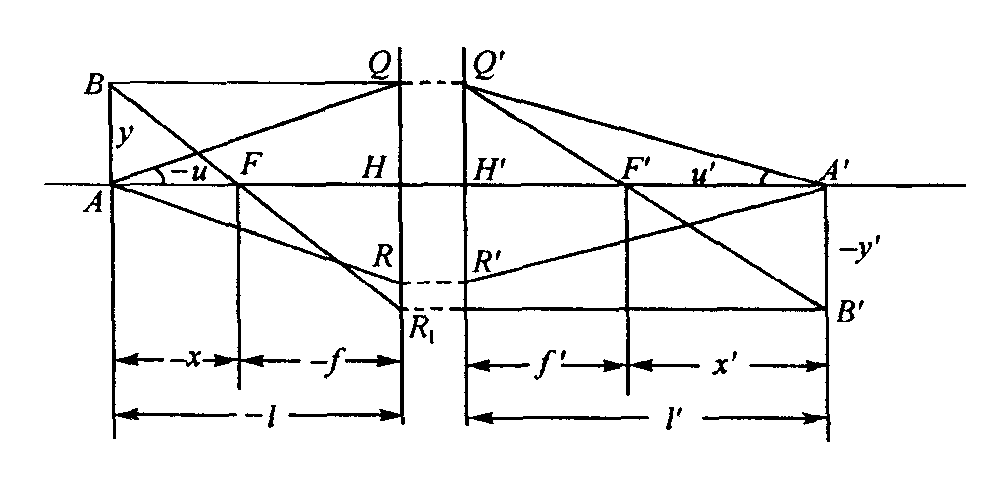
\includegraphics[width=0.7\textwidth]{newton-and-gauss.png}
	\caption{理想光学系统}
	\label{newton-and-gauss}
\end{figure}

如图\ref{newton-and-gauss}所示,由相似三角形可导出
\begin{equation}
xx'=ff'
\label{newton-eq-1}
\end{equation}
\begin{equation}
\beta=\frac{y'}{y}=-\frac{x'}{f'}=-\frac{f}{x}
\label{newton-eq-2}
\end{equation}
式(\ref{newton-eq-1})为牛顿公式,以焦点为原点。式(\ref{newton-eq-2})为牛顿公式的垂轴放大率公式。

\subsection{高斯公式}
如图\ref{newton-and-gauss}所示,焦物距、焦像距和物距、像距之间有如下关系:
\begin{equation}
\begin{cases}
x=l-f\\
x'=l'-f'
\end{cases}
\end{equation}
将其带入牛顿公式(\ref{newton-eq-1}),两边同时除以$ll'$可得
\begin{equation}
\frac{f'}{l'}+\frac{f}{l}=1
\label{gauss-eq-1}
\end{equation}
式(\ref{gauss-eq-1})为高斯公式,以主点为原点。其相应的垂轴放大率公式为
\begin{equation}
\beta=\frac{y'}{y}=-\frac{f}{f'}\frac{l'}{l}
\label{gauss-eq-2}
\end{equation}
当物方介质和像方介质相同时,有$f'=-f$,则式(\ref{gauss-eq-1})和式(\ref{gauss-eq-2})可以写成
\begin{equation}
\frac{1}{l'}-\frac{1}{l}=\frac{1}{f'}
\end{equation}
\begin{equation}
\beta=\frac{l'}{l}
\end{equation}

\subsection{两焦距之间的关系}
在近轴光线区域,$fyu=-f'y'u'$,共轴球面系统的近轴区适用拉赫公式$nyu=n'y'u'$,则可得出物方焦距和像方焦距之间的关系式:
\begin{equation}
\frac{f'}{f}=-\frac{n'}{n}
\end{equation}
若光学系统中包括反射面,则两焦距之间的关系由反射面个数决定。设反射面个数为$k$,则有
\begin{equation}
\frac{f'}{f}=(-1)^{k+1}\frac{n'}{n}
\end{equation}
理想光学系统的拉赫公式为
\begin{equation}
ny\tan U=n'y'\tan U'
\label{lah-eq}
\end{equation}

\section{理想光学系统的放大率}
前面已经给出垂轴放大率的公式(\ref{newton-eq-2})和(\ref{gauss-eq-2}),下面给出轴向放大率和角放大率。
\subsection{轴向放大率}
物平面沿光轴移动$\mathrm{d} x$或$\mathrm{d} l$时,像平面移动$\mathrm{d} x'$或$\mathrm{d} l'$,轴向放大率为
\begin{equation}
\alpha=\frac{\mathrm{d} x'}{\mathrm{d} x}=\frac{\mathrm{d} l'}{\mathrm{d} l}
\end{equation}
微分可得
\begin{equation}
\alpha=-\frac{x'}{x}
\end{equation}
将式(\ref{newton-eq-2})带入得
\begin{equation}
\alpha=-\beta^2\frac{f'}{f}=\frac{n'}{n}\beta^2
\end{equation}

\subsection{角放大率}
角放大率为
\begin{equation}
\gamma=\frac{\tan U'}{\tan U}
\end{equation}
根据理想光学系统拉赫公式(\ref{lah-eq})得
\begin{equation}
\gamma=\frac{n}{n'}\frac{1}{\beta}
\end{equation}
理想光学系统三种放大率之间的关系为
\begin{equation}
\alpha\gamma=\beta
\end{equation}
\subsection{光学系统中的节点}
\label{subsect:node}
\begin{definition}{节点}{int}
	光学系统中角放大率等于$+1^{\times}$的一对共轭点为节点。
\end{definition}

\begin{property}
	光线通过节点方向不发生改变。
\end{property}

\begin{problem}
	正透镜对虚物成像时:
	\begin{itemize}
		\item [(a)] 只能成实像
		\item [(b)] 只能成虚像
		\item [(c)] 只能成缩小像
		\item [(d)] 只能成放大像
	\end{itemize}
\end{problem}

\begin{solution}
	选择(a)和(c)。
\end{solution}

\begin{problem}
	光学系统的节点是:
	\begin{itemize}
		\item [(a)] 垂轴放大率为$1$的共轭点
		\item [(b)] 角放大率为$1$的共轭点
		\item [(c)] 物方发出过物方节点的光必经过像方节点
		\item [(d)] 物方发出过像方节点的光必经过物方节点
	\end{itemize}
\end{problem}

\begin{solution}
	选择(b)和(c)。
\end{solution}

\begin{problem}
	某物方、像方介质相同的折射光学系统对物成像时有$-1<\beta<0$,则当物体向透镜移动时有:
	\begin{itemize}
		\item [(a)] 像向透镜移动
		\item [(b)] 像远离透镜移动
		\item [(c)] 像移动速度比物快
		\item [(d)] 像移动速度比物慢
	\end{itemize}
\end{problem}

\begin{solution}
	选择(b)和(d)。
\end{solution}

\section{理想光学系统的图解求像}
\elegantpar{画光路图}{图解求像是考试中必考的题目,而且所占分值很多,这一类的题需要多练,如果熟练掌握的话,完全是送分题,否则就是送命题}的依据:
\begin{enumerate}
	\item 平行于光轴的光线经理想光学系统后必通过像方焦点;
	\item 过物方焦点的光线经理想光学系统后必为平行于光轴的光线;
	\item 过节点的光线方向不变;
	\item 任意方向的一束平行光经理想光学系统后必交于像方焦平面上一点;
	\item 过物方焦平面上一点的光线经理想光学系统后必为一束平行光;
	\item 主面交点光线高度相同。
\end{enumerate}

\begin{exercise}\label{draw-beam-path-1}
	已知二光组基点,由物求像或由像求物。
	\begin{figure}[htbp]
		\centering
		\includegraphics[width=0.8\textwidth]{draw-beam-path.pdf}
	\end{figure}
\end{exercise}

\begin{note}
	在这一类绘制光路图的题中,需要注意过第二个透镜光轴处的辅助线与过第一个透镜到其焦面$F_1$的光线平行,这一条线要交于第二个透镜的焦面$F_2$处,经过该交点与光线和第二个透镜的交点的线即为出射光线。
\end{note}

\section{理想光学系统的组合}
\label{sect:combination-of-optical-systems}
\begin{figure}[htbp]
	\centering
	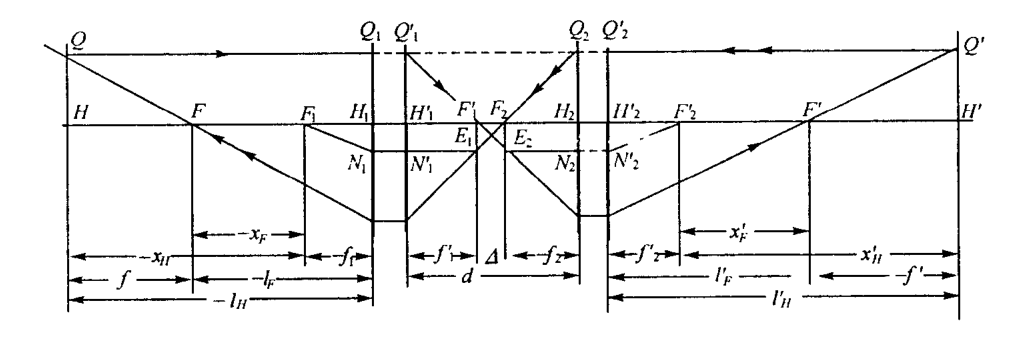
\includegraphics[width=1\textwidth]{combination-of-optical-systems.png}
	\caption{两个光组的组合}
	\label{combination-of-optical-systems}
\end{figure}

图\ref{combination-of-optical-systems}给出了由两个光组组成的等效系统在两个空间的焦点和主点。按牛顿公式,物焦距$x=-\Delta$,其焦像距$x'_F$为
\begin{equation}
x'_F=-\frac{f_2f'_2}{\Delta}
\end{equation}
同理有
\begin{equation}
x_F=\frac{f_1f'_1}{\Delta}
\end{equation}
根据相似三角形$\triangle Q'H'F'\sim\triangle N'_2H'_2F'_2$和$\triangle Q'_1H'_1F'_1\sim\triangle E_2F_2F'_1$,可导出
\begin{equation}
f'=-\frac{f'_1f'_2}{\Delta}
\end{equation}
同理有
\begin{equation}
f=\frac{f_1f_2}{\Delta}
\end{equation}
大多数情况下光学系统位于空气中,应有$f'_1=-f_1$,$f'_2=-f_2$和$f'=-f$。所以有
\begin{equation}
\Delta=d-f'_1+f_2=d-f'_1-f'_2
\end{equation}
则有
\begin{equation}
f'=-f=\frac{f'_1f'_2}{f'_1+f'_2-d}
\end{equation}
表示成光焦度形式为
\begin{equation}
\phi=\phi_1+\phi_2-d\phi_1\phi_2
\end{equation}

\begin{definition}{折合距离与光焦度}{int}\label{def:focal-power}
	一线段的长度除以该线段所在介质的折射率做得的值称为该线段的折合距离。折合焦距的倒数称之为光学系统的光焦度,以$\Phi$表示,即
	\begin{equation}
	\Phi=\frac{n'}{f'}=-\frac{n}{f}
	\end{equation}
	如果光学系统位于空气中,其光焦度用$\phi$表示,即
	\begin{equation}
	\phi=\frac{1}{f'}=-\frac{1}{f}
	\end{equation}
	光焦度的单位是折光度或屈光度。正光焦度的光学系统对光束起会聚作用;负光焦度的光学系统对光束起发散作用。
\end{definition}

根据图\ref{combination-of-optical-systems},还可得到如下关系:
\begin{equation}
\begin{cases}
l'_F=f'_2+x'_F,\quad l_F=f_1+x_F\\
l'_H=l'_F-f',\quad l_H=l_F-f
\end{cases}
\end{equation}
据此可得出等效系统基点相对于主点的位置关系。

等效系统的放大率$\beta$仍可用基本公式$\beta=-f/x$计算。$f$为等效系统的焦距,$x$为物点到等效系统的物方焦点距离,得到
\begin{equation}
\beta=\frac{f_1f_2}{f_1f'_1-x_1\Delta}
\end{equation}

\section{望远镜系统}

\begin{definition}{望远镜系统}{int}
	使入射的平行光束仍保持平行地出射的光学系统称为望远镜系统。望远镜系统的焦距无穷大,焦点和主点位于无穷远。
\end{definition}

\begin{figure}[htbp]
	\centering
	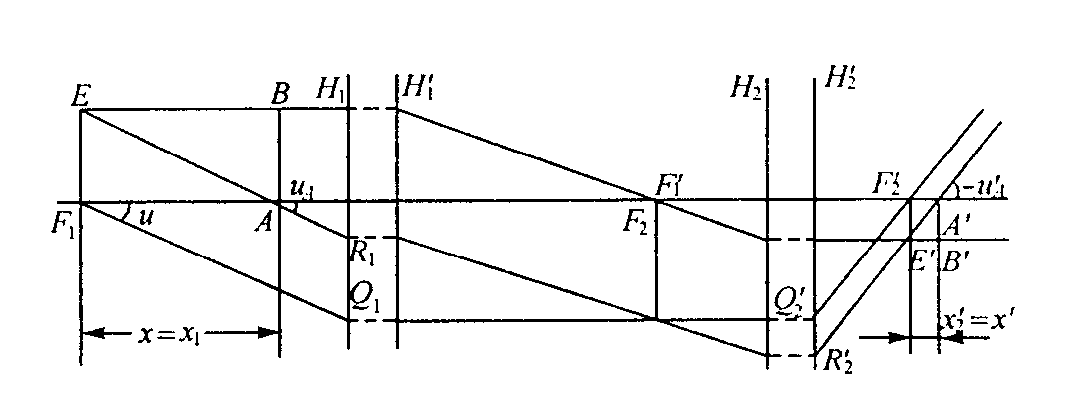
\includegraphics[width=0.7\textwidth]{telescope-system.png}
	\caption{望远镜系统}
	\label{telescope-system}
\end{figure}

如图\ref{telescope-system}所示,根据牛顿公式,并考虑过渡公式$\Delta=0$,可导出
\begin{equation}
x'_2=\frac{f_2f'_2}{f_1f'_1}x_1
\end{equation}
\begin{equation}
\beta=\beta_1\beta_2=\frac{f_2}{f'_1}
\end{equation}
轴向放大率公式为
\begin{equation}
\alpha=\frac{\mathrm{d}x'_2}{\mathrm{d}x_1}=\frac{f_2f'_2}{f_1f'_1}
\end{equation}
角放大率为
\begin{equation}
\gamma=\frac{\tan u'}{\tan u}=\frac{f_1}{f_2}
\end{equation}
在空气中,$f'_1=-f_1$,$f'_2=-f_2$,因此有
\begin{equation}
\beta=-\frac{f'_2}{f'_1}
\end{equation}
\begin{equation}
\alpha=\beta^2
\end{equation}
\begin{equation}
\gamma=-\frac{f'_1}{f'_2}=\frac{1}{\beta}
\end{equation}
\begin{equation}
x'_2=\alpha x_1
\end{equation}
由此可见,望远镜系统的各种放大率,仅由组成该系统的两个光组的焦距决定。

供眼睛观察用的光学系统为目视光学系统,目视光学系统中最重要的参数为视觉放大率。
\begin{definition}{望远镜系统的视觉放大率}{int}\label{def:visual-magnification}
	望远镜系统的视觉放大率是远处物体经系统所成的像对眼睛张角$W'$的正切与该物体直接对眼睛张角$W$的正切之比,用$\Gamma$表示。望远镜系统的视觉放大率等于该系统的角放大率,即
	\begin{equation}
	\Gamma=\frac{\tan W'}{\tan W}=\gamma=-\frac{f'_1}{f'_2}=\frac{1}{\beta}
	\end{equation}
	所以,望远镜系统的视觉放大率是物镜焦距与目镜焦距之比。
\end{definition}

一个有限焦距系统之前加角放大率为$\Gamma$的望远镜系统时,整个系统的焦距为原焦距的$\Gamma$倍,即
\begin{equation}
f'=\Gamma f'_2
\end{equation}

\section{透镜}
\subsection{薄透镜}

\begin{definition}{薄透镜}{int}
	透镜的厚度与球面半径相比很小,略去厚度不会引起成像结果的实质性变化,却能对初始阶段的分析和计算带来方便,导出简单的公式。这时认为透镜的厚度为零,称薄透镜。
\end{definition}

薄透镜的物像位置公式:
\begin{equation}
\frac{1}{l'}-\frac{1}{l}=(n-1)\bigg(\frac{1}{r_1}-\frac{1}{r_2}\bigg)
\label{thin-lens}
\end{equation}
焦距为
\begin{equation}
f'=\frac{1}{(n-1)\bigg(\frac{1}{r_1}-\frac{1}{r_2}\bigg)}
\end{equation}
并有$f=-f'$。其光焦度为
\begin{equation}
\phi=\frac{1}{f'}=(n-1)\bigg(\frac{1}{r_1}-\frac{1}{r_2}\bigg)
\end{equation}
则式(\ref{thin-lens})可以写成
\begin{equation}
\frac{1}{l'}-\frac{1}{l}=\frac{1}{f'}=\phi
\end{equation}

由此可知,凸透镜焦距为正,光焦度为正,对光束起会聚作用,像方焦点是对入射平行光束会聚而成的实焦点。凹透镜焦距为负,光焦度为负,对光束起发散作用,像方焦点为虚焦点。因此称凸透镜为正透镜或会聚透镜,凹透镜为负透镜或发散透镜。

通过
\begin{equation}
\beta=\frac{f'}{l+f'}
\end{equation}
可以得出,当$\beta=1$时,解得$l=0$,此时一对物像点重合于薄透镜的中心或顶点,角放大率为$1$,表示这一对共轭点共轭光线有相同方向。因这对共轭点重合于薄透镜中心,所以过薄透镜中心的光线方向不变。

\begin{property}
	薄透镜具有下列性质:
\begin{enumerate}
	\item 平行于光轴入射的光线经透镜后通过像方焦点;
	\item 过物方焦点的入射光线经过透镜后平行于光轴射出;
	\item 通过透镜中心的光线方向不变。
\end{enumerate}
\end{property}

\subsection{厚透镜}
对于几种常见的厚透镜的讨论:
\begin{enumerate}
	\item 双凸透镜:保持两面的半径不变,随着厚度$d$的不同,其焦距可正可负。当$d<|n(r_2-r_2)/(n-1)|=M$时,$f'$为正,光线会聚,两个主面总位于透镜内部;当$d=M$时,$f'=\infty$;当$d>M$时,$f'$为负,主面在透镜外。
	\item 双凹透镜:$f'$恒为负,发散透镜,两主面位于透镜内部。
	\item 平凸透镜:$f'$恒为正,其值与透镜厚度无关,两主面上的一个相切于球面的顶点,另一个位于透镜内部。
	\item 平凹透镜:$f'$恒为负,其值与透镜厚度无关,两主面上的一个相切于球面的顶点,另一个位于透镜内部。
	\item 弯月形凸透镜:$f'$恒为正,若凸面朝向物方,则物方主面在凸面之前,像方主面在凹面之前,二者都在透镜外。
\end{enumerate}
	
\end{document}